\documentclass{mimosis}
\usepackage{graphicx} % Required for inserting images
\graphicspath{ {./images/} }
\usepackage{amsmath}
\usepackage{amsfonts}
\usepackage{mathtools}
\usepackage[square,authoryear]{natbib}
\usepackage{hyperref}
\hypersetup{
	colorlinks = true,
	urlcolor = RoyalBlue,
	linkcolor = RoyalBlue,
	citecolor = RoyalBlue
}

\usepackage[noabbrev, capitalize]{cleveref}
\usepackage{booktabs}
\setlength{\parindent}{0pt} % Don't indent paragraphs
\usepackage{parskip}
\usepackage{algorithm}
\usepackage{algpseudocode}
\usepackage{tikz}


\usepackage{caption} % for \captionof --> allows for non-float tables and figures
\usepackage{array,multirow,makecell}
\setcellgapes{1pt}
\makegapedcells
\newcolumntype{R}[1]{>{\raggedleft\arraybackslash }b{#1}}
\newcolumntype{L}[1]{>{\raggedright\arraybackslash }b{#1}}
\newcolumntype{C}[1]{>{\centering\arraybackslash }b{#1}}


\usepackage{babel}
\usepackage{microtype}

\usepackage{placeins} %for \FloatBarrier to force tables and figures to appear exactly where asked

\KOMAoptions{twoside=false, DIV=12, BCOR=7mm} % manage line width automatically depending on font size, equal size for RV

%\allowdisplaybreaks

%\title{Makespan Minimization of the Job Shop Scheduling Problem Constrained by Conflict Graph}
%\author{Augustin Martignoni}
%\date{}

\begin{document}

%\maketitle

\begin{titlepage}

\begin{tikzpicture}[remember picture,overlay]
   \node[anchor=north east,inner sep=20pt] at (current page.north east)
              {\includegraphics[scale=1]{UNF_Logo_100pr_pos.jpg}};
\end{tikzpicture}

  	\begin{center}
		\vspace*{2cm}
  		\begin{huge}
  			Travail de Bachelor \\
  		\end{huge}

  		\vspace{1cm}
    
  		\begin{LARGE}
  			 Makespan Minimization of the Job Shop Scheduling Problem Constrained by Conflict Graph 
  		\vspace{0.5cm}
	\end{LARGE}
  	\end{center}

  	\begin{center}
  		\begin{Large}
  			Augustin Martignoni \\ 
  		\end{Large}
  		\vspace{1.5cm}
  		\date{}
  	\end{center}

  	\vspace{1.5cm}
  	\begin{tabular}{L{4cm}l}
		Université	& Université de Fribourg\\
				&\\
  		Faculté 	& Faculté des sciences et\\
				& de médecine\\
				&\\
  		Département & Département d'informatique\\
				& DS\&OR Group\\
				&\\
  		Noms des & Prof. Bernard Ries \\
		superviseur.e.s & Dr. Nour Elhouda Tellache \\
						& \\
  		Nom de l'étudiant.e & Augustin Martignoni \\
  		Numéro d'étudiant.e & 16-214-546\\
  		\\
  		& \\
		&  \\
		\\
  	
  	\end{tabular}
  \end{titlepage}

\tableofcontents

%\section{Abstract}
%In job shop scheduling problems with conflict graphs, we have a set \(\mathcal{J} = \{J_j, j = 1, \dots, n\}\) of \(n\) jobs that has to be processed on a given set \(\mathcal{M} = \{M_i, i = 1, \dots, m\}\) of \(m\) dedicated machines, and a simple undirected graph \(\mathcal{G} = (V, E)\) over the jobs, called the conflict graph. Each job \(J_j\) consists of \(m_j\) operations \(O_{aj}^{i_a}\) \((a = 1, \dots, m_j)\), where \(O_{aj}^{i_a}\) is the \(a\)-th operation of job \(J_j\), to be processed on machine \(i_a\) for \(p_{aj}\) time units. The processing times \(p_{aj}\) are non-negative numbers. Two operations belonging to the same job cannot be processed at the same time and each machine can process at most one job at a time. On the other hand, each vertex in \(G\) represents a job, and two operations of different jobs on different machines cannot be processed at the same time (meaning they are in conflict) if and only if the jobs they belong to are adjacent in \(G\). The objective is to find a feasible schedule that minimizes the makespan \(C_{\text{max}}\), i.e., the overall time needed to process all the jobs. When the operations of each job must be processed in a predefined order, the model is referred to as Job Shop with Conflict graph (JSC).

\chapter*{Abstract}
\addcontentsline{toc}{chapter}{Abstract}
\markboth{}{Abstract}

This work proposes the Job Shop Scheduling Problem augmented by Conflict Graph (JSC), an extension of classical Job Shop Scheduling Problem. In this problem, conflicts between tasks (that cannot be treated at the same time on different machines) are introduced in the form of a simple, undirected graph on the tasks. We propose a mathematical model for this problem in the form of a Mixed-Integer Linear Problem (MILP). For this problem, we propose lower bounds that take advantage of this new graph element, and a genetic algorithm, a heuristic inspired from natural evolution, tailored to the JSC. We then use benchmark instances based on well-known instances for the Job Shop Scheduling Problem, and showcase the limits of the MILP when solved with a commercial solver. Computational experiments also highlight the performance of conflict-based lower bounds, as well as the capability of the genetic algorithm to quickly find a good quality solution to the JSC even for large test instances.

\chapter*{Introduction}
\addcontentsline{toc}{chapter}{Introduction}
\markboth{}{Introduction}

The field of scheduling, in which one assigns ressources to perform tasks, is everywhere. Finding an optimal schedule can lead to less time waste in a factory, less movements of students and professors between classes, or a more performant computer (when scheduling program processes).

Common problems in this field include the Job Shop Scheduling Problem (hereafter JSSP), where the operations of each task must be processed on different machines in a specific order, different for each tasks. The JSSP has been widely studied since its infancy in the middle of the last century, with applications in many fields such as metallurgy \citep{yang2016pareto}, rail transport \citep{buergy2016blocking_rail_bound}, the chemical industry \citep{gao2016shuffled}, semiconductor manufacturing \citep{panwalkar2016proportionate}, and many more.

However, the basic JSSP is only concerned about making sure no operation of a task is being assigned before the previous operation of the same task is complete, and ensuring no two operations are processed on the same machine at the same time. Each operation can only be processed on specific machines, and the order of the operations, while fixed, is different from task to task. The objective of this process is to ensure we find the smallest possible completion time of the last operation to be scheduled, also known as makespan.

This is already a very difficult and time-consuming problem to solve optimally when the total number of operations and machines becomes large enough. Indeed, the problem is NP-Hard, with the time to solve it growing exponentially as the number of tasks and machines grows larger. This however doesn't account for additional conflicts between operations. Modeling conflicts between operations, such as two different courses being taught by the same teacher, or two metallic parts needing the specially-trained machinist, makes solving the problem even harder. 

To offer a potential solution to this matter, we model the conflicts between tasks using a simple undirected graph, which we call a conflict graph. The problem is referred to as Job Shop Scheduling Problem constrained by Conflict Graph (hereafter JSC).

The first chapter of this work will offer a brief theoretical introduction to the topics of scheduling and graph theory. This is to offer a general understanding of the problem, and establish some definitions for important concepts used in the later chapters.

The second chapter will provide a formal definition of the JSC in the form of a mathematical model, as well as introduce lower bounds and a genetic algorithm for the JSC.

Finally, the last chapter of this work will showcase the environment and parameters for our experiments. This will be followed by the results of the mathematical formulation solved by a commercial solver, as well as an evaluation of the performance of several lower bounds for the JSC. A last section will cover the results of our proposed genetic algorithm for the JSC.

\chapter{Generalities and Definitions}

As this work relies on several mathematical and computer science concepts, It is appropriate to formally present them in this section. This will refresh the reader's knowledge, and aid in understanding the content that follows. Examples will be included to demonstrate the real-world relevance of these concepts.

The aim of this chapter is however not to give a detailed explanation of the concepts, but indeed to introduce the main theoretical base for the next chapters in a light and easily understandable manner. As such, this chapter is a condensate of several sources, notably \emph{Handbook of Scheduling: From Theory to Applications}, by \citet{blazewicz2007handbook},  and \emph{Scheduling: Theory, Algorithms, and Systems}, by \citet{pinedo2008scheduling}.

\section{Scheduling Theory}

This work features the subject of scheduling, and as such, it is important to give a brief introduction to the concepts used in this work. To its core, scheduling concerns the assignment of resources, which can be factory machines, workers or classrooms, but also processing units in a computer, to tasks to be accomplished, like manufacturing part of an object, hosting the professor and students of a particular course, or in the case of the CPU of a computer, executing tasks.

Scheduling theory is the branch of mathematics and computer science that studies such problems, which are often non-trivial and require a significant amount of time and computing power to solve. Indeed, a lot of these problems are NP-hard, which means the time taken to solve grows at least exponentially with the size of the input \citep{garey1979computers}. It is also interested in the development of algorithms and methods to solve them efficiently according to a set goal, like maximizing the number of parts manufactured per hour, or minimizing the student and professor movements between classes.

\subsection{Components of machine scheduling}

%% add definition of machine scheduling --> wait for relecture --> not really needed, comes further

The main components of machine scheduling can be summarized as follows.

\subsubsection{Tasks}

Tasks are the primary element of scheduling problems. They represent the work to be accomplished, and are the elements to be scheduled. A scheduling problem contains habitually a certain number of tasks, often accompanied by a processing time that indicates how much time the task takes to accomplish.

\subsubsection{Resources}

Whereas tasks represent activities that need to be accomplished in order for the machine scheduling problem to be solved, resources represent the elements that process the tasks. They also represent auxiliary resources which might be needed to process a task. Taking again the example of a school, the tasks, lectures, are "processed" by classrooms, with the help of a professor, the resources.

\subsubsection{Constraints}

Constraints are restrictions on the machine scheduling problem. They represent guidelines that must be respected when building the schedule.

Constraints can be of several types. Some are temporal, meaning they impose a restriction on task precedence, task due dates and task release times. Other constraints are related to the ressources.

As an example, one of the most common type of constraints aims to ensure that resources do not process more tasks at any one time than their capacity allows for (e.g. ensuring that, in an airport, no two aircraft are parked in a stand at the same time).

Continuing on the example of the school, possible constraints may range from making sure that a professor is available whenever they are scheduled to teach, to making sure that if a two time slots long lecture is scheduled in a classroom during a particular time slot, the same classroom is also reserved for the same lecture in the next time slot. This could also include making sure that no dual-slot lectures are scheduled over a lunch break.

\subsubsection{Objective functions}

Objective functions are the last element of a scheduling problem we will highlight. Where tasks and resource define the elements of the problem, and constraints add context and rules to produce a meaningful schedule, 

Objective functions define the criteria for the problem to be solved optimally. Resolution methods make sure to solve the scheduling problem according to these criteria, or at least provide a feasible solution, if an optimal solution cannot be found. It is possible for a scheduling problem to have several parameters that define the optimality of the solution, and therefore have several objective functions accordingly.

The most common objective function consists in minimizing the maximum completion time of all tasks, but there exist many more, like minimizing idle time for a resource.

Returning to our school example, several objective functions are possible, with the trivial option being maximizing the number of lectures scheduled. Another objective could involve minimizing student movements between classes, or minimizing the number of half-days where each professor teaches.

\subsection{Machine Scheduling Environments} % since machine scheduling

Machine scheduling is a broad class of optimization problems, that aim to create a \emph{schedule}, an assignment of tasks, to resources, which are designated as \emph{machines}. As this nomenclature tends to indicate, a common application of this class of problems is found in the optimization of factories or assembly lines. Their purpose is to create a schedule that assigns machines to process tasks. 

Machine scheduling is typically split into two subclasses, parallel and dedicated scheduling, the main differentiator between those two classes being the numbers of \emph{operations}, steps, in a task. Parallel scheduling problems consider single-operation tasks, which can be run on any machine, while the tasks of dedicated scheduling problems have multiple steps.

\subsubsection{Single Machine}

First is the simple case of there being only one machine. This case may be considered as a reduction to one machine of the identical parallel machines case, which we will treat below. It should be noted that most problems of the single machine type can be solved very efficiently using algorithms that are very efficient \citep{lawler1993sequencing}.

\subsubsection{Parallel scheduling}
Parallel Scheduling is commonly split into three classes depending on the speed of the machines. 

\paragraph{Identical parallel machines}
First is the case where all machines are identical, meaning each machine completes a task in \emph{exactly} the same time as another machine would complete the same operation. 

One can imagine several cases where such a situation occurs, and one example could be found in an array of completely identical computers, who will all execute the same piece of code in exactly the same time.

\paragraph{Uniform parallel machines}

A second case occurs when all machine are uniform. This is defined similarly to the above case of identical machines. However, each machine is now given a \emph{speed factor}, and will therefore be generally slower or faster than another machine. This speed factor does not depend on the tasks.

In practice, this can cover several events, and some examples could cover machines of the same model, but of different ages and worn in different amounts, or machines of the same type but of different brands, or maybe machines in need of different amounts of maintenance, or maybe all of them at once.

For consistency with the previous section, let us imagine an array of computers of the same model and brand, but with some of them having a reduced cooling efficiency because of dust.

\paragraph{Unrelated parallel machines}

Finally, as an even more general case, we find the unrelated machines. All can execute the same tasks, but a machine will be able to execute one particular task faster than an other machine, but could be slower than the same other machine at executing another operation. This means that, unlike the uniform machines case, the speed factor is now dependent on the tasks.

Continuing on the example of computers, this time let us consider an array of computers not filled with computers of different brands, models, some with faster CPUs, some others also configured with graphics processing units, some even with specialized accelerators, all of different ages and in different stages of maintenance. It is easy to see that there will be no consistency in the speed difference for all tasks in any two of the computers. All machines are therefore unrelated.

One can easily see that the case of the unrelated machines is therefore a generalization of the uniform machines case, which is itself a generalization of the identical machines case.

\subsubsection{Dedicated Scheduling}

Dedicated scheduling, as with parallel scheduling and its variants, is split into three main categories. Where before, in parallel scheduling, all machines were able to execute any task, the tasks are now separated into dedicated \emph{operations}, which must be executed on a particular machine. Hence, the machines are now dedicated and can only process certain operations. 

As the tasks in a dedicated scheduling problem are composed of multiple independent operations, each needing to be processed on a particular machine, the distinction between those categories is found in the ordering imposed on the operations.

\paragraph{Open Shop}

First in the dedicated scheduling section, we find the open shop. This type of scheduling problem, while imposing a restriction on the machine an operation can be executed on, doesn't impose a restriction on the processing order of a task's operations, and they can be executed at any time.

This type of situation can often occur in manufacturing where multiple independent elements have to be added to a product. One can for example consider the manufacturing of a printed circuit board, where most electronic components must be installed and soldered by a specialized machine, but the order in which they are added in doesn't matter.

\paragraph{Flow Shop}

A second case concerns the flow shop. This type of machine scheduling problem can be seen as a restriction of the open shop scheduling problem, as the only distinction between the two is that the flow shop requires the operations of each task to follow a precise processing order, which is identical for all tasks.

This type of problem arises when the steps to manufacture a product are not independent, with each operation requiring the previous operations to be completed first. Some manufacturing lines operate in this manner, as each step in the fabrication of an end product depends on the last. One can indeed not create colored pencils without first adding the dye to the wax that will make the core of the pencil. However, the process doesn't change if the dye or the length of the final pencils changes.

One can probably think of the steps required to produce nearly any common product on their desk and obtain a problem in the form of a flow shop, but an example that particularly highlights this need for a precise ordering in the fabrication of medicines, where all processing happens in chemical reactor, and each reaction requires a previous component.

\paragraph{Job Shop}

The final case of dedicated scheduling is found in the job shop. The job shop is a further restriction on the flow shop, and while very similar to it, it differs in the fact that the operations of each task can take a different order on the machines. As such, an implicit restriction is that no two successive operations of the same task cannot be executed on the same machine (as they would otherwise be combined into one, and their processing times added together).

A good example of such a process is a manufacturing shop taking very diverse orders from many customers. We can consider a machining shop, where the quantity, size, material and features of each order may require multiple operations on different machines, different for each piece.

\subsubsection{Classification of scheduling problems}

In order to more easily denote the properties of scheduling problems, \citeauthor{graham1979optimization} established in a now famous paper \citep{graham1979optimization} a standard classification, and accompanying notation. This eponymous Graham notation, also referred to as the \emph{three-field notation}, is written \(\alpha \mid \beta \mid \gamma\).

\paragraph{\(\alpha\) field}
The first field gives information upon the machine environment of the problem. It is split into two characters \(\alpha_1\) and \(\alpha_2\). It gives information on the general type of machine scheduling problem, and the number of machines in said problem.

\begin{description}
\item \(\alpha_1\) indicates the type of problem, and can be any of the elements of the set \(\{P,Q,R,\circ,O,F,J\}\), representing respectively Identical parallel machines, Uniform parallel machines, Unrelated parallel machines, Single machine, Open shop, Flow shop and Job shop.
\item \(\alpha_2\) indicates the number of machines, and can be either \(\circ\) or a positive integer \(m\). The latter case implies that the number of machines is constant, and the former indicates a variable number of machines. Additionally, we have that \(\alpha_1 = \circ \iff \alpha_2 = 1\).
\end{description}

\paragraph{\(\beta\) field}
This second field is commonly split into six fields, numbered \(\beta_1,...,\beta_6\). They give indications on the characteristics of the tasks.

\begin{description}
\item \(\beta_1\) indicates whether \emph{preemption}, that is interrupting the processing of an operation, and resuming it later, is allowed.
\item \(\beta_2\) indicates the presence or absence of a limitation on the resources. Should such a limitation exist, it also implies the existence of data highlighting the number of resources necessary for each task during its processing.
\item \(\beta_3\) allows for the specification of an order on the tasks, meaning preventing the processing of the operations of a task until the one or more tasks it depends on have finished processing.
\item \(\beta_4\) specifies the \emph{release date} of each task, meaning the time until each task can begin processing. If this information is not present, we assume that all tasks are released for processing at time \(0\).
\item \(\beta_5\) allows, in the case of \(\alpha_1 = J\), the specification of a constant upper bound on the number of operations in each task.
\item \(\beta_6\) concerns the processing times of all operations of all tasks, and allows for the definition of constant upper and/or lower bounds on the processing time of all operations, or even to declare that all operations are all processed in \(1\) time unit. 
\end{description} 

Since this second field concerns task characteristics, the above list in non-exhaustive, and variants on the above fields are often used, depending on the specific problem one is treating.

%%ask here
\paragraph{\(\gamma\) field}
This paragraph concerns optimality criteria, or in other words, the objective function or functions one chooses to optimize the problem for. These objective functions are computed for each specific schedule, and offer a way to find which schedule is the best, according to each optimality criterion.

Several parameters can be extracted from a schedule. For example, one can compute, for each task \(i\), the completion time \(C_i\), the lateness (the difference between the completion time and the due date) \(L_i\), or even the task penalty (\(0\) if the task is on time, \(1\) if it late). One typically refers to the maximal lateness as \(Lmax\), and to the maximal completion time, or \emph{makespan}, as \(Cmax\). 

\(\gamma\) is typically a minimization of the \(Cmax\) or the \(Lmax\), but many varieties of optimization criteria can be found, depending on the problem. Some scheduling problems optimize for example the total energy use or the total environmental impact of the tasks.

\paragraph{Extension}

Because of the evolution of the machine scheduling field, the three-field notation has been expanded many times, according to the needs of the researchers using it. We will ourselves define and employ our own extension to the three-field notation further in this work.

\subsection{Gantt diagram} 
Scheduling problems, for communication and visualization purposes, sometimes need to be graphically represented. This is accomplished in the form of a Gantt chart. This type of chart plots the schedule by showing which task (when dealing with parallel machines) or operation (when dealing with dedicated machines) is processed on each machine at each time. One draws a box whose length is proportional to the processing time of each task respectively each operation, starting at the position where it starts processing on the axis of time.

An example is given in \cref{fig:7_7-JSSP-Gantt}, which shows a Gantt chart for a job shop scheduling problem, with 7 machines and 7 tasks, each task containing 7 operations.

%\FloatBarrier
\begin{figure}[H]
\includegraphics[width=15cm]{7_7-test_0.0_1.png} %% !! replace by 7x7 test image.
\centering
\captionof{figure}{An example of a Gantt chart, for a scheduling problem of type \(J7||Cmax\)}
\label{fig:7_7-JSSP-Gantt}
\end{figure}
%\FloatBarrier

\subsection{Resolution methods}
As we get to a larger scale, that is, the number of machines and/or the number of operations per task becomes larger. Finding an exact solution to machine scheduling problem using exact methods becomes therefore impractical, due to the computational complexity of the problem. 

One therefore needs to find a method that is guaranteed to generate a close-to-optimal schedule in a time-efficient way. This type of method is called a \emph{heuristic}. While heuristics doesn't necessarily lead to finding an optimal solution, they are able to efficiently search space of all feasible solutions without checking every single one. This allows them to quickly converge towards a solution that performs close to the optimal solution. One can also find \emph{metaheuristics}, which are methods that are able to adapt and guide common heuristics to improve their performance. These metaheuristics are often inspired from real-life phenomena, such as natural evolution, or the annealing of metals.

Several types of heuristics and metaheuristics exist, but the most common for solving machine scheduling problem include
\begin{itemize}
\item Local search, which considers an initial feasible solution, and applies small modifications to it to potentially find an improved solution in its neighbors (similar solutions). If an improved solution is found, it becomes the new current solution. This cycle continues until a time limit, iteration limit or other criterion has been reached.
\item Tabu search, which is a metaheuristic that extends local search, proposed by \citet{glover1986, glover1989}. Tabu search prevents revisiting solutions that have previously been tried. It also adds a mechanism by which a worse solution can be adopted if no better solution is available. This prevents the search from being stuck in a local minimum.
\item Genetic algorithms, which were introduced by \citet{holland1975adaptation}, mimic the natural process of evolution. They maintain a population of feasible solutions (chromosomes), which evolve over successive iterations. At each iteration, solutions are evaluated using a fitness function, and new individuals (children) are created through the recombining of parent solutions, and mutation. By eliminating bad performing solutions and favoring ones that perform well, the algorithm converges slowly to a near-optimal solution.
\end{itemize} 

\section{Graph Theory}
Graph theory is the field of mathematics and computer science concerned with the study of abstract structures called graphs. 
It is interested in their properties and their applications to problems, as well as the design and study of algorithms to efficiently solve them. 


The word graph, in the mathematical sense, refers to an abstract structure comprised of vertices and edges that represent relationships between objects \citep{schrijver2003}. An example graph is shown in \cref{fig:graph_example}.

\begin{figure}[h!]
    \centering
    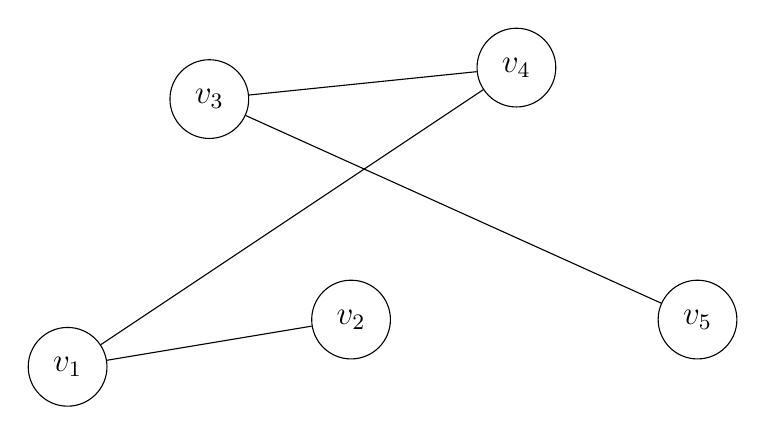
\begin{tikzpicture}[scale=2, every node/.style={circle, draw, minimum size=10mm, font=\large}]
        % Vertices
        \node (A) at (0,-0.3) {\(v_1\)};
        \node (B) at (1.8,0) {\(v_2\)};
        \node (C) at (0.9,1.4) {\(v_3\)};
        \node (D) at (2.85,1.6) {\(v_4\)};
        \node (E) at (4,0) {\(v_5\)}; 

        % Edges
        \draw (A) -- (B);
        \draw (C) -- (E);
        \draw (A) -- (D);
        \draw (C) -- (D);
    \end{tikzpicture}
    \caption{Example graph with 5 vertices and 4 edges}
    \label{fig:graph_example}
\end{figure}

\subsection{Graphs and their general properties}

Several types of graphs can be found in graph theory. However, the graphs used in this work are only of the simple, undirected category. Hence, we will going forward refer to the simple, undirected graphs as graphs.

Formally, a graph is a pair \( G = (V, E) \), where:

\begin{itemize}
    \item \( V \) is a finite set of elements \( v_i \), called \emph{vertices}, or sometimes \emph{nodes};
    \item \( E \) is a finite set of pairs \( \{v_k, v_l\} \) with \( v_k, v_l \in V \); the elements of \( E \) are called \emph{edges}.
\end{itemize}

Two vertices connected by an edge are called \emph{adjacent}, and a vertex \( v_i \) is \emph{incident} to an edge \( e \in E \) if \( v_i \in e \).

It is also important to highlight two properties of vertices. For a vertex \( v \in V \), we call:

\begin{itemize}
    \item \( \deg(v) \) the \emph{degree} of \( v \), where \( \deg(v) \) is equal to the number of edges incident to \( v \);
    \item \( N(v) \) the \emph{neighborhood} of \( v \), where \( N(v) \) is the set of all vertices adjacent to \( v \) in \( G \).
\end{itemize}

We can see that, in the case of simple, undirected graphs, we have that \(\forall v \in V \), \( |N(v)| = \deg(v) \).

The definition of a graph is very general, highlighting its purpose as a representative tool. It is the graph's user's purpose to assign meaning to the vertices and to the edges linking them together, when applying a graph construction to a set of data. Hence, a family tree, in which the vertices, family members, are adjacent if they are related by a parent–child relationship, is a graph representing the links between families. But a graph can also be used to represent bus stops, and whether they are served by the same bus line, or atoms of a molecule, and whether two atoms are linked by a direct chemical bond. A graph is a universal tool applied to real-world situations to model objects and their relations. This helps in representing these objects in a simpler way, or to solve problems on these objects.

\subsection{Complement of a graph}

Since, in a graph \( G = (V, E) \), the edges indicate connections of some type between vertices, their absence indicates the lack of such a connection. 
Such a lack of connections can be represented by the \emph{complement} of \( G \). 
The complement \( \overline{G} = (V, \overline{E}) \) of  \( G \) is defined as follows:

\[
    \overline{E} = \big\{ \{v_k, v_l\} \mid v_k, v_l \in V, \, v_k \neq v_l, \, \{v_k, v_l\} \notin E \big\}.
\]

The vertices of \( \overline{G} \) are the same as those of \( G \), but its set of edges is comprised of the set of all possible edges that can be created between the vertices of \( V \), without the edges contained in \( E \).

\subsubsection{Adjacency matrix} % IMPORTANT !!!

One further property of graphs is their ability to be represented as a matrix, if one makes abstraction of the node names. 
This is useful in several programming tasks where checking the adjacency of two vertices is important, including this work. 
Such a representation is called an \emph{adjacency matrix}, and works as follows:

Assume we have a graph \( G = (V, E) \), as previously defined. 
The adjacency matrix of \( G \), denoted generally as \( A \), is a binary \( |V| \times |V| \) matrix defined as

\[
A_{i,j} =
\begin{cases}
1, & \text{if } \{v_i, v_j\} \in E, \\
0, & \text{otherwise}.
\end{cases}
\]

Since there are no edges going from one vertex to itself in a simple graph, we further have that \( A_{i,i} = 0, ~\forall \space v_i \in V \).

It should be noted that, as long as the ordering of vertices is the same for both the columns and the rows of \( A \), the specific ordering does not matter, and does not change the underlying graph.

\subsection{Node-weighted graphs}

Sometimes, a simple undirected graph is not quite enough to represent the full extent of real-world objects. 
Indeed, what about the example of the previous section talking about molecules? 
It is trivial to see that, unless a molecule is composed of exactly one type of atom, the graph representation is not sufficient. 
It would therefore be interesting to have, for a vertex representing an atom, a complementary weight representing the atomic weight of the atom, or maybe the atomic number of the atom, as an example.

This can be done by assigning to each vertex \( v_i \in V \) a weight \( w_i \in \mathbb{R} \). 
As explained above, like in the case of vertices and edges, the problem-specific meaning of vertex weights heavily depends on what the user seeks to represent. 
They simply expand further the modeling power of graphs.

\subsection{Independent set problem}

Just as important as finding relations between objects, it is also important to be able to find objects that are not directly related. 
In a graph \( G = (V, E) \), a subset \( V' \subseteq V \) of vertices, where
\[
\forall v_i, v_j \in V', \; \{v_i, v_j\} \notin E,
\]
is called an \emph{independent set}. 
A graph can contain several independent sets, and an independent set as large as or larger than any other independent set in the same graph is called a \emph{maximum independent set}. 
In general, finding a maximum independent set in a graph is a difficult task to accomplish with exact methods, and such a problem requires approximate methods to solve in reasonable time.

\subsection{Greedy heuristics for the weighted independent set problem} %% maybe not as a new section

Since finding an exact solution to the maximum independent set problem is difficult, finding the maximum weight independent set in a weighted graph is also difficult, and requires the use of a heuristic.

We opted to use the GWMIN and GWMIN2 greedy heuristics, as defined by \citet{sakai2003note}. These two algorithms work in two steps. They first compute a score for each vertex of the graph, select the node with the highest score, and add the selected node to the weighted independent set. The selected node and its neighborhood are then removed from the graph, and the algorithm repeats until there are no vertices left in the graph. These heuristics are greedy, because they select the best scoring vertex at each step.

GWMIN and GWMIN2 differ slightly in their scoring function. While GWMIN computes the score of each vertex by dividing its weight by its degree, GWMIN2 computes the score of each vertex by dividing the weight of a vertex by the sum of the weights of all vertices in its neighborhood and its own weight.

\chapter{Job Shop Scheduling Problem with Conflict graph}

\section{Problem description}
The standard job shop scheduling problem, hereafter JSSP, is noted using the three-field notation as \(Jm \mid\mid C_{\text{max}}\). We have a fixed number \(m\) of machines, on which \(n\) tasks, \(J_1, \dots, J_n\), must be executed. Each of these tasks is composed of an ordered sequence of operations \(O_{ij}^{m_{ij}}\), such that \(J_j = \{O_{1j}^{m_{1j}}, \dots, O_{nj}^{m_{nj}}\}\). This notation means that the \(i\)-th operation of task \(J_j\) is executed on machine \(m_{ij}\). This notations is further augmented by two matrices, \(P = p_{(ij)}\) and \(M = m_{(ij)}\), where \(p_{(ij)}\) is the processing time of operation \(O_{ij}^{m_{ij}}\), \(m_{(ij)}\) the machine it is executed on. Additionally, from the definition of the JSSP comes the facts that only one operation can be processed at the same time on each machine, and that a task can only be processed on only a single machine at a time. As an objective function, we minimize the total makespan (\(C_{max}\)) For simplification, we restrict our JSSP to \(m\) operations per task, with each task containing exactly one operation per machine. It should however be noted that this does not prevent the application of the methods described in this work to less restrictive implementations of the JSSP.

We add to our problem the notion of a conflict graph, resulting in the JSSP augmented with conflict graph, hereafter JSC, which we denote as \(Jm \mid ConfG \mid C_{max}\) in the three-field notation. \(ConfG = (V,E)\) is a simple undirected graph with \(n\) vertices \(v_1, \dots, v_n\), that each correspond to a single task. If \(v_k\) and \(v_l\) are adjacent in \(ConfG\), then the corresponding tasks \(J_k\) and \(J_l\) are \emph{in conflict}, and no operation of either task can be processed while an operation of the other task is being processed. \(ConfG\) is represented by its adjacency matrix \(A = a_{(ij)}\), where \(a_{(kl)} = a_{(lk)} = 1\) if and only if tasks \(J_k\) and \(J_l\) are in conflict.

The JSSP can be solved using several methods, either exhaustive or approximative. Examples of exhaustive methods include a mathematical modeling of the JSSP in the form of equations and inequalities, with one or more objective functions to optimize. This mathematical model can then be solved with numerical methods, usually by using a solver, a dedicated program specialized in solving constraint problems, to exhaustively search the solution space of the equation set. Such a solver usually uses techniques like the branch-and-bound algorithm.

However, such techniques also suffer from an increase in solving time, such that it becomes impractical to use exact methods to solve these problems. Indeed, while some particular cases of the JSSP can be solved efficiently \citep{blazewicz2007handbook}, \citet{sotskov1995nphardness} showed that the JSSP with three tasks and three operations per task is already NP-hard, meaning that the general \(n\)-tasks, \(m\)-machines case is also NP-hard. As a further consequence, the JSC with \(n\)-tasks and \(m\)-machines is also NP-hard for arbitrary conflict graphs.

\section{Mathematical formulation} \label{sec:mathmodel}
In order to mathematically model the the JSC, we extend and adapt the JSSP formulation proposed in \citet{blazewicz2007handbook}. 
We denote with \(O_0\) and \(O_{\text{last}}\) the artificial first respectively last operations of all tasks, with \(p_0\) and \(p_{\text{last}}\) equal to \(0\).

Let \(\mathcal{M}\) denote the set of \(m\) machines and \(\mathcal{A}\) be the set of ordered pairs \((O_{lj}^{i_l},\ O_{(l+1)j}^{i_{l+1}})\) of tasks constrained by the precedence relations \(O_{lj}^{i_l} \prec O_{(l+1)j}^{i_{l+1}}\) for each task.

For each machine \(M_k\), the set \(\mathcal{E}_k = \{(O{aj}^{i_a},\ O_{(a+1)j}^{i_{a+1}}) : J_j \in \mathcal{J},\ a \leq m_j - 1\}\) describes the set of all pairs of tasks that must be executed on this machine, and are therefore unable to be processed concurrently.

For each operation \(O_{lj}^{i_l}\), the corresponding processing time \(p_{lj}\) is fixed, and the earliest possible starting time of \(O_{lj}^{i_l}\) is \(t_{lj}\) is a decision variable that has to be determined during the optimization. Hence, the job shop scheduling problem can be modeled as:
\begin{align}
\text{Minimize } \quad & t_n \label{eq:objective} \\
\text{subject to} \quad 
&t_{(a+1)j} - t_{aj} \ge p_{aj} 
&& \forall\, (O_{aj}^{i_a}, O_{(a+1)j}^{i_{a+1}}) \in \mathcal{A}
\label{math-model-precedence-constraint} \\
&t_{aj} - t_{bl} \ge p_{bl} - (1 - \delta_{aj,bl}^{machine}) \cdot M
&& \forall\, (O_{aj}^{i}, O_{bl}^{i}) \in \mathcal{E}_i,\ 1 \le i \le m
\label{math-model-machine-constraint-bigM1} \\
&t_{bl} - t_{aj} \ge p_{aj} - \delta_{aj,bl}^{machine} \cdot M
&& \forall\, (O_{aj}^{i}, O_{bl}^{i}) \in \mathcal{E}_i,\ 1 \le i \le m
\label{math-model-machine-constraint-bigM2} \\
&\delta_{aj,bl}^{machine} \in \{0,1\}
&& \forall\, (O_{aj}^{i}, O_{bl}^{i}) \in \mathcal{E}_i,\ 1 \le i \le m
\label{math-model-delta-machine} \\
&t_{lj} \ge 0 
&& \forall\, O_{lj}^{i_l},\ 1 \leq l \leq m,\ 1 \leq j \leq n
\label{math-model-nonnegative-constraint}
\end{align}
First, the inequalities (\ref{math-model-precedence-constraint}) establish precedence constraints. They ensure that an operation of a task cannot be scheduled until the preceding operation has finished processing. Formally, we ensure this property by requiring that the starting time of an operation be greater or equal to the sum of the starting time and the processing time of the operation that precedes it.

Secondly, we ensure with the inequalities (\ref{math-model-machine-constraint}) that no more than one operation can be scheduled on any machine at the same time. 

This is done by requiring that, for any two operations that must be processed on the same machine, the difference between the starting time of the second to be scheduled and that of the first to be scheduled must be greater or equal to the processing time of the first to be scheduled. Since either of the operations can be scheduled before the other, we are left with the inequalities (\ref{math-model-machine-constraint}).
\begin{align} 
\label{math-model-machine-constraint}
t_{aj} - t_{bl} \geq p_{bl} \quad &\text{or} \quad t_{bl} - t_{aj} \geq p_{aj} \quad \forall \, (O_{aj}^{i},\ O_{bl}^{i}) \in \mathcal{E}_i,\ 1 \leq i \leq m
\end{align} 
As the solver program we will use further in this work doesn't understand this type of disjunction, we need to split it into two inequalities. This can be done using the big M method, with \(M = \sum_{(i,j) \in [1, m] \times [1, n]} p_{ij} + 1\), the sum of all processing times of all operations, plus 1. This notation adds for each set of inequalities a binary decision variable (\ref{math-model-delta-machine}), that subtracts M from the right side of only one of the inequalities (\ref{math-model-machine-constraint-bigM1}) and (\ref{math-model-machine-constraint-bigM2}). This makes one of these inequalities always satisfied, as the differences \(t_{bl} - t_{aj}\) and \(t_{aj} - t_{bl}\) mathematically cannot be larger than \(M\).

The solver is therefore left with the choice of which inequality to consider, which amounts to deciding which of the two operations will be processed first. The downside of this method is that we need to add a decision variable for each pair of operations that are on the same machine. In our case, with exactly one operations per machine per task, this means inserting \(m * (n^2 - n)\) additional decision variables. This naturally augments the complexity of the JSSP even further.

Finally, it should be noted that in the present state, the starting times can be negative, which we do not want. Thus, we require in the inequalities (\ref{math-model-nonnegative-constraint}) that all the starting times be greater than or equal to 0.

These restrictions ensure that the predetermined processing order of operations is respected, that only one task can be processed on one machine at a time, and that all tasks are completed. However, In order to consider the effect of the conflict graph applied to the JSSP, additional constraints need to be appended to the above formulation. 

Let \(ConfG = (V, E)\) be a conflict graph, with \(V = \mathcal{J}\), and a pair of tasks \((J_k, J_l)\) being adjacent if they are in conflict. In order to avoid repeating constraints, we only consider those operations in conflict that occur on different machines and belong to different tasks. 

Since we operate on operations rather than on tasks, we define the additional set  
\[ 
C = \{(O_{aj}^{i_a}, O_{bl}^{i_b}) : j \ne l,\ J_j, J_l \in \mathcal{J},\ (J_k, J_l) \in E,\ 1 \leq a \leq m_j,\ 1 \leq b \leq m_l,\ a \neq b\}, 
\]
that contains all pairs of operations in conflict. 

To account for the conflicts in the mathematical model of the JSSP, and thereby convert it into a JSC, we define the inequalities (\ref{math-model-conflict-constraint}), that operate very similarly to inequalities (\ref{math-model-machine-constraint}), replacing the \(\mathcal{E}_i\) sets by \(C\).
\begin{align} 
\label{math-model-conflict-constraint}
t_{aj} - t_{bl} \geq p_{bl} \quad \text{or} \quad t_{bl} - t_{aj} \geq p_{aj} \quad \forall\, (O_{aj}^{i_a},\ O_{bl}^{i_b}) \in C
\end{align} 
We note however that this is also a disjunction of inequalities, which we again need to transform using the big M method. We use the same value of M as for the machine conflicts to add inequalities (\ref{math-model-conflict-constraint-bigM1}) and (\ref{math-model-conflict-constraint-bigM2}).
\begin{align}
&t_{aj} - t_{bl} \ge p_{bl} - (1 - \delta_{aj,bl}^{conflict}) \cdot M
&& \forall\, (O_{aj}^{i_a}, O_{bl}^{i_b}) \in C
\label{math-model-conflict-constraint-bigM1} \\
&t_{bl} - t_{aj} \ge p_{aj} - \delta_{aj,bl}^{conflict} \cdot M
&& \forall\, (O_{aj}^{i_a}, O_{bl}^{i_b}) \in C
\label{math-model-conflict-constraint-bigM2} \\
&\delta_{aj,bl}^{conflict} \in \{0,1\}
&& \forall\, (O_{aj}^{i_a}, O_{bl}^{i_b}) \in C
\label{math-model-delta-conflict-binary}
\end{align}
\section{Lower bounds} \label{Lower bounds}
While finding an optimal solution to the JSSP using exact methods is computationally intensive, it is however possible to find lower bounds for the makespan of the JSSP. We will further compare the following methods to see which provides the best lower bound, and in which cases one method may perform better than another.

\subsection{Solver-provided lower bounds}
Solver programs used to solve mathematical programming problems usually compute lower bounds for the problem they are trying to solve during their execution. It is therefore easy to extract these values for further use. The solver used for the experiments in  \cref{chapter:experiments} provides such a lower bound for the makespan.

\subsection{Trivial bounds}
Due to the properties of the JSSP, some trivial bounds are very simple to compute. First, the makespan of a JSSP instance will never be lower than the sum of all processing times of any task. That is, we have that :
\begin{equation} \label{task_lower_bound_equ}
C_{max} \geq \max_{1 \leq j \leq n} \sum_{s = j} p_{is}
\end{equation}
We can therefore compute the sum of the execution times of all operations of each task, and take the maximum of those values as a trivial lower bound.

Similarly, an identical process can be applied to the machines. We have that :
\begin{equation} \label{machine_lower_bound_equ}
C_{max} \geq \max_{1 \leq l \leq m} \sum_{p \in M_l} p,\ M_l = \{p_{ij} \mid O_{ij}^{m_l} \text{ is processed on machine }m_l, 1 \leq j \leq n, 1 \leq i \leq m\}
\end{equation}
Thus, computing the sum of the execution times of all operations on each machine, and taking the maximum of those values also grants us another trivial lower bound.

\subsection{Conflict-based bounds}
Since the JSC adds conflicts between tasks, meaning none of the operations of tasks in conflict can be scheduled together, it makes sense that adding the processing time of all operations of the maximal number of tasks in conflict together will produce a lower bound. 

This task reduces to the problem of finding the maximum weighted clique of a graph, which is itself computationally expensive. Finding these bounds therefore requires heuristic methods. We use two algorithms \emph{GWMIN} and \emph{GWMIN2}, introduced by \citet{sakai2003note}, on the complement of our conflict graph, with the nodes weighted by the total processing time of each task. 

This provides us another two lower bounds, which may differ slightly due to the different node selection criteria between the two algorithms in question.

\section{Genetic Algorithms}

State of the art methods among the metaheuristics that have been successfully applied to JSC often use genetic algorithms to find close-to-optimal solutions in a short time \citep{xiong2022survey}. We have accordingly chosen to develop such a metaheuristic to apply to the JSC.

Genetic algorithms \citep{holland1975adaptation} are inspired by the natural evolution process, and often follow a schema similar to the following overview of the Genetic Algorithm we will use for the JSC.

\begin{enumerate}
\item a \emph{population} of potential solutions, \emph{chromosomes} are generated. These individuals are represented in our case as \(m\) permutations of the operations of each machine.
\item all chromosomes are evaluated using a fast heuristic, and classified according to the relevant criterion, in our case the makespan.
\item one or more pairs of chromosomes are selected to evolve further.
\item each pair of chromosomes undergoes \emph{crossover}, in which \emph{children} are created by taking a portion of a chromosome, and completing the rest of the child with the \emph{genes} of the other chromosome. 
\item with a certain probability, a \emph{mutation} can be applied to a child chromosome in order to further modify it and distinguish from its parents.
\item all children are then evaluated with the same heuristic as used to initially evaluate the population, and either some or all of the population is replaced by the new children. The process then starts again at step 3.
\end{enumerate}

This schema is very adaptable, and the next section will showcase our implementation of this schema.

\section{A Genetic Algorithm for the JSC}

\subsection{Chromosome representation}

To simplify the function of the genetic algorithm, we represent a chromosome, a potential solution to an \(M\)x\(N\) JSC instance, as \(M\) sets of operations, one for each machine, that each contain a permutation of all operations for each specific machine. Each operation is represented as a tuple \(\{i, j, p_{ij}\}\).

\subsection{Initial population} \label{Initial population}
We opted to test several variants for the selection of the initial population. First is the number \(n\) of individuals. We tested variants with \(n = \{100, 200, 300\}\). Concerning the generation of the chromosomes, we enforced a restriction such that no two chromosomes would have an identical makespan, to ensure diversity in the population. Two variants for the generation of the population were tested. The first generates an entirely random population, and the second, which we refer to as semi-heuristic, augments a number of pre-determined chromosomes with random chromosomes, generated similarly to those of the first method. These deterministic chromosome are composed as follows :
\begin{enumerate}
\item For each operation \(O_{ij}^{m_{ij}}\), we select the processing time \(p_{ij}\). For each sub-chromosome, we order the operations by processing time, first in descending order for a first chromosome, and then ascending for a second.
\item For each operation \(O_{ij}^{m_{ij}}\), we compute the \emph{conflict degree} \(c_{ij}\), which is the number of operations it is in conflict with. For each sub-chromosome, we order the operations by conflict degree, first in descending order for a first chromosome, and then ascending for a second.
\item For each operation \(O_{ij}^{m_{ij}}\), we retrieve the \(p_{ij}\) and \(c_{ij}\), then compute \(c_{ij} \div p_{ij}\). Again, for each sub-chromosome, we order the operations these new values, first in descending order for a first chromosome, and then ascending for a second.
\end{enumerate}

\subsection{Chromosome evaluation} \label{Chromosome evaluation}
For each chromosome, we generate a schedule and compute its makespan. This is done using \cref{nondelay-heur-alg}, adapted from \citep{tellache2023genetic}, that creates a non-delay schedule. This means that the schedules created by this algorithm will ensure that a machine will not be kept idle, should it be possible to schedule an operation on it. This property makes it highly likely that our genetic algorithm will converge towards an optimal solution, though it should be noted that the optimal schedule is not guaranteed to be non-delay.

%\FloatBarrier
\begin{algorithm}
\begin{spacing}{1.2}  % force 1.2 line spacing within the algorithm
\captionof{algorithm}{Building a non-delay schedule} \label{nondelay-heur-alg}
\begin{algorithmic}[1]
\Require Set \(\pi\) of permutations \(\pi_{1}, \ldots, \pi_{m}\) of operations, processing times \((p_{ij})_{1 \leq i \leq n,\ 1 \leq j \leq m}\), adjacency matrix \(A\) of \(\text{ConfG}\)
\State Initialise the earliest starting times \((s_{ij})_{1 \leq i \leq n, 1 \leq j \leq m}\) of all operations to \(0\)
\While{\(\pi \neq \{\emptyset\}\)}
    %% maybe not random ? modify if needed
    \State Randomly select an operation \(O_{ij}^{m_k}\) with the minimum earliest starting time \(s_{ij}\), among the list of first operation of each permutation \(\pi_k\), \(1 \leq k \leq m\) with this earliest starting time.
    \State Compute \(c_{ij} = s_{ij} + p_{ij}\), the \emph{completion time} of operation \(O_{ij}^{m_k}\)
    \State \(\pi_k \gets \pi_k \setminus \{O_{ij}^{m_k}\}\)
    \ForAll{operations \(O_{ab}^{m_l}\) in \(\pi_l\), \(1 \leq l \leq m\), that are in conflict with \(O_{ij}^{m_k}\)}
        \If{\(s_{ab} < s_{ij} + p_{ij}\)}
            \State \(s_{ab} \gets s_{ij} + p_{ij}\)
        \EndIf
    \EndFor
\EndWhile
\Statex \textbf{Output:} Starting times \((s_{ij})_{1 \leq i \leq n, 1 \leq j \leq m}\) and the makespan
\end{algorithmic}
\end{spacing}
\end{algorithm}
%\FloatBarrier

\subsection{Chromosome selection}

For the selection of a chromosome, we decided to select a single pair. Selection is delicate : while it is tempting to simply take the best and second best chromosome in the population, or the best and the worst, this in practice means the algorithm converges too fast as well as improperly, potentially converging far from the optimal solution. We must therefore take a probabilistic approach.

We first order the chromosomes by makespan, in the descending order. Note that since we ensure that no two individuals have the same makespan, there is no need to make a decision as to which equivalently performing chromosome should be sorted first. We then assign to each chromosome the parameter \(k\), which corresponds to the rank of the chromosome in the newly created order.

Selection of the first chromosome then aims to select a solution that is biased towards the best performing chromosomes, to avoid regression. Accordingly, each chromosome has a probability \(p_{1} = \frac{2k}{N(N+1)}\) of being chosen as the first element of the crossover pair.

The selection of the second chromosome should however be equally likely to select a good- or bad-performing chromosome, and each chromosome besides the one chosen in the previous step therefore has an uniform probability \(p_{2} = \frac{1}{(N-1)}\) of being selected as the second element of the crossover pair.

\subsection{Crossover} \label{crossover}
Crossover is the crucial part of a genetic algorithm. Since we are considering crossover over permutations, we need to use crossover operators that respect their ordering.

We evaluate several traditional crossover operators : 
\begin{itemize}
\item Partially Mapped Crossover (PMX) \citep{goldberg1985alleles}, in which we select two positions, and take the segment in between these two positions from the first parent chromosome. The remainder of the child chromosome is filled by taking the genes outside of the crossed segment from the second parent in order. If the current gene is already present in the child chromosome, we consider the gene in the second parent that is at the same position as the current gene in the first parent. Repeat this procedure until a gene not present in the child chromosome is found. 
\item Order Crossover (OX1) \citep{davis1985applying}, which starts like PMX, but then simply creates the remainder of the child from the genes of the second parent, inserting them sequentially (while skipping those already present) after the copied section.
\item Finally, Linear Order Crossover (LOX) \citep{oliver1987study} is a variant of OX1, where the insertion of genes from the second parent starts at the beginning of the child chromosome.
\end{itemize}

All three operators rely on the selection of two points to apply a crossover operation to the chromosomes. Since in the case of the JSSP and JSC, the chromosomes are sets of permutations, we adapt the operators to successively apply to each permutation in the first chromosome and its counterpart in the second chromosome, as described in \cref{crossover-application-alg}. For each pair of permutations, a different pair of crossover points is randomly chosen.

%\FloatBarrier
\begin{algorithm}
\begin{spacing}{1.2}  % force 1.2 line spacing within the algorithm
\captionof{algorithm}{Application of a crossover operator to a set of permutations} \label{crossover-application-alg}
\begin{algorithmic}[1]
\Require Two sets \(\{\pi_{a1}, \ldots, \pi_{am}\}\) and \(\{\pi_{b1}, \ldots, \pi_{bm}\}\) of permutations
\State Initialize sets \(\{\chi_{a1}, \ldots, \chi_{am}\}\) and \(\{\chi_{b1}, \ldots, \chi_{bm}\}\)
\For{\(l = 1\) to \(m\)}
    \State Generate two random crossover points \(\lambda, \mu\) such that \(1 \leq \lambda < \mu \leq m\)
    \State Apply a crossover operator to \(\pi_{al}\) and \(\pi_{bl}\) using positions \(\lambda\) and \(\mu\) to produce two child permutations \(\chi_{al}\) and \(\chi_{bl}\)
    \State Store \(\chi_{al}\) and \(\chi_{bl}\) in their respective sets
\EndFor
\Statex \textbf{Output:} Two sets of child permutations \(\{\chi_{a1}, \ldots, \chi_{am}\}\) and \(\{\chi_{b1}, \ldots, \chi_{bm}\}\)
\end{algorithmic}
\end{spacing}
\end{algorithm}
%\FloatBarrier

Note that all three methods can create two children from two parents, depending on which parent is chosen first. We consider both children, and randomly select one for further mutation. 

\subsection{Mutation} \label{mutation}
Mutation allows us to introduce in chromosomes variations that have either been forgotten during the evolution process, or are not present in the population in the first place, through local search. Mutation in consequence widens the search space coverage of the genetic algorithm, while also preventing premature convergence by ensuring the genetic algorithm can escape from local minima \citep[p.~110]{holland1975adaptation}. Since mutation naturally occurs randomly which a small probability, we choose to set the mutation probability \(p_{mut}\) of our genetic algorithm to \(p_{mut} = 0.2\). 

We further evaluate two common mutation operators :
\begin{itemize}
\item SWAP, which exchanges two randomly chosen genes.
\item MOVE, which takes a randomly chosen gene, and inserts it in another place, thus shifting a part of the permutation to the right.
\end{itemize} 

\subsection{Replacement}
We are left with one new child chromosome, which we need to insert in the population. We first evaluate the child to ensure the value of its makespan isn't already present in the population, in which case we discard it. We then randomly select with uniform probability a chromosome among the lowest-performing (highest makespan) section of the population, and replace it with the new child chromosome.

\subsection{Stopping criteria}

Without interruption, a genetic algorithm will continue to evolve, even if no further change is applied to the population. We thus decide to provide three stopping criteria, which are based on feedback from the algorithm, as well as reasonable limits.

First is a limit on the maximum number of iterations, which is modular, based on the population size PS as well as the greater of the number of machines and the number of tasks, multiplied by a factor of 1000 \citep{tellache2023genetic}. We compute this \emph{max\_iter} stopping criterion based upon the formula :
\begin{equation} \label{max_iter_equ}
max\_iter = PS \cdot \max \{n,m\} \cdot 1000
\end{equation}
It should be however noted that none of our tests reached a million iterations, but an adaptive max\_iter may become relevant for larger instances. 

While max\_iter is a hard criterion, the next two criteria are based upon feedback from the genetic algorithm itself. Second in the list of criteria is \emph{max\_tries}, a limit on the maximum number of consecutive tries of the genetic algorithm that do not result in an improvement of the makespan of the best solution. 

This in practice means the absence of a change to the best makespan found so far, and often indicates the genetic algorithm has converged to a close-to-optimal solution. We set \(\emph{max\_tries} = 1000\), which is large enough to prevent the inherent randomness of a genetic algorithm from triggering this condition earlier than expected.

Finally, we retrieve the best lower bound among all those computed using the methods described above, and configure the genetic algorithm to stop if this lower bound is reached. In this case, the best computed solution would be optimal, and continuing the execution of the algorithm further would not provide any improvement.

\subsection{General framework}

To provide a better view of the genetic algorithm, we provide within this section \cref{alg:genetic-schema}, a high-level overview of the different steps used in this work. 

\begin{algorithm}[H]
\begin{spacing}{1.2}
\captionof{algorithm}{General schema of the genetic algorithm used in this work}
\label{alg:genetic-schema}
\begin{algorithmic}[1]
\Require Lower bound \(L\), operations \(O_{ij}^{m_{ij}}\), \(1 \leq i \leq m, 1 \leq j \leq n\), their processing times \(p_{ij}\), adjacency matrix \(A\) 
\State Generate initial population of chromosomes, each represented as a set of permutations [\emph{See \cref{Initial population}}]
\While{\(\text{best\_}C_{\max} > L\) \textbf{or} \(\text{curr\_iter} < \text{max\_iter}\) \textbf{or} \(\text{curr\_reps} < \text{max\_reps}\)} [\emph{See \cref{Lower bounds}}]
    \State Compute \(C_{\max}\) for all chromosomes using a non-delay heuristic [\emph{See \cref{Chromosome evaluation}}]
    \State Sort chromosomes by \(C_{\max}\) in descending order
    \State Probabilistically select two chromosomes according to \(p_1\) and \(p_2\)
    \State Perform crossover on the two selected chromosomes [\emph{See \cref{crossover}}]
    \State Randomly choose one child chromosome from the crossover
    \If{random() \(< p_{\text{mut}}\)}
        \State Apply mutation to the chosen child chromosome [\emph{See \cref{mutation}}]
    \EndIf
    \State Replace one chromosome from the lower-performing half of the population with the new child chromosome
\EndWhile
\Statex \textbf{Output:} Optimal or near-optimal schedule and its \(C_{\max}\)
\end{algorithmic}
\end{spacing}
\end{algorithm}

It should be noted, however, that this method can be modified in several ways, with maybe better performance, most notably with different crossover operators, additional heuristics, or by completely replacing the population at each step by performing crossover on \(\frac{N}{2}\) pairs of chromosomes.


\chapter{Computational experiments} \label{chapter:experiments}

\section{Context} 

In this chapter, we evaluate the performance of the mathematical model, lower bounds, and genetic algorithm using instances derived from the literature. The first section will describe the instances used in the tests, followed by an evaluation of the lower bounds. We then cover the mathematical model and, finally, discuss the genetic algorithm, by determining the parameters that need to be fixed for the tests, then evaluating the overall performance of the algorithm.\footnote{The code used to generate the results used in this work can be found on the author's \href{https://github.com/amartignoni/JSC_makespan_minimization_bachelor_thesis}{Github account}.}

\section{Test instances}

We test our various algorithms on instances derived from the JSSP instances provided by \citet{taillard1993benchmarks}. These instances have size \[(n,m) \in \{(15,15),(20,15),(20,20),(30,15),(30,20),(50,15),(50,20),(100,20)\}.\] 
%% add a bit more on Taillard instances
for each of the test instances, nine conflict graphs were generated, three each of low, medium, and high conflict density, to represent the JSC with different amounts of conflict. These graphs are generated on vertices each representing a task, using the Erdös-Rényi \citep{erdos1959random} method. Accordingly, any edge between two vertices is included in the conflict graph \(ConfG\) with a probability \(p\). We choose \(p \in \{0.2, 0.5, 0.8\}\), depending on the desired conflict density.  

\section{Lower bounds} \label{sec:exp_lower_bounds_results}

We first want to consider which lower bound algorithm produces the best lower bound. We decided to present all our results separated by conflict graph density. We first notice that the lower bound computed by a solver (see \cref{sect:mathmodel}) is in most cases the best-performing method, especially for lower and medium density conflict graphs, as can be seen in \cref{tab:lbprob02}, \cref{tab:lbprob05} and \cref{tab:lbprob08}. Where this solver lower bound isn't the most performant, it is superseded by the GWMIN and GWMIN2 algorithms. These algorithms, differing only by their node ranking formulas, provide identical results for all the JSC instances covered in this work. We will therefore only refer to GWMIN thereafter, but it should be understood as "GWMIN and GWMIN2", except where explicitly stated otherwise.

The results we obtained for the performance of each lower bound are presented in \cref{tab:lbprob02}, \cref{tab:lbprob05} and \cref{tab:lbprob08}. These tables show the percentage of the total test instances of each size where the task with the largest total processing time (JLB), the machine with the largest total processing time (MLB), GWMIN, GWMIN2, and the solver-provided lower bounds provided the best lower bound. Note that in case of an equality, the instance was counted for all tied lower bounds. As such, the sum of all percentages on each line doesn't equal to \(100\%\).

Differences appear mostly in the instances with a conflict graph of large density, where the conflicts become the biggest limiting factor in computing the Cmax. Due to their nature, the lower bounds generated by the GWMIN algorithms start competing with those computed by the solver. GWMIN outperforms the algorithms between 15\% and 25\% of all instances with 15 machines. However, the biggest surprise lies in the results obtained in the high-density instances with 20 machines, where all instances are better bounded by the GWMIN algorithms than the solver (with the exception of the \(100\)x\(20\) instances). This effect is likely due to the fact that the GWMIN algorithms can find a larger weight independent set due to the larger number of operations in each task.

Of note is the fact that the trivial lower bounds do not perform well for all instances of the JSC. The presence of even a low-density conflict graph dramatically increases the lower bound of the problem, beyond what can be reached by considering the machine with the biggest combined operating time or the task with the biggest combined processing time. With these trivial lower bounds not taking the conflicts into account, our results highlight this criterion as a requirement for an algorithm to provide a good lower bound for the JSC.

We also note that for most instances, even those where the solver-computed lower bound is better, the GWMIN-computed lower bound is a close second, far ahead of the trivial methods of computing the lower bound. Additionally, while the solver may provide the best lower bound in many cases, especially for low and medium conflict densities, this performance comes at the cost of a higher CPU time. Furthermore, we observed no difference in the results between GWMIN and GWMIN2, but such a difference may exist in practice. We would therefore encourage the use of both algorithms in parallel, then taking the best result of the two, as their computation is both cheap and fast.

%\FloatBarrier
\begin{table}[h]
\centering
\begin{tabular}{c|ccccc}
NxM & JLB & MLB & GWMIN LB & GWMIN2 LB & Solver LB \\
\hline
15x15 & 0.0\% & 0.0\% & 0.0\% & 0.0\% & 100.0\% \\
20x15 & 0.0\% & 0.0\% & 0.0\% & 0.0\% & 100.0\% \\
20x20 & 0.0\% & 0.0\% & 0.0\% & 0.0\% & 100.0\% \\
30x15 & 0.0\% & 0.0\% & 0.0\% & 0.0\% & 100.0\% \\
30x20 & 0.0\% & 0.0\% & 0.0\% & 0.0\% & 100.0\% \\
50x15 & 0.0\% & 0.0\% & 0.0\% & 0.0\% & 100.0\% \\
50x20 & 0.0\% & 0.0\% & 0.0\% & 0.0\% & 100.0\% \\
100x20 & 0.0\% & 0.0\% & 0.0\% & 0.0\% & 100.0\% \\
\end{tabular}
\captionof{table}{Percentage of instances with probability \(p = 0.2\) where each algorithm found the best lower bound}
\label{tab:lbprob02}
\end{table}
%\FloatBarrier

%\FloatBarrier
\begin{table}[h]
\centering
\begin{tabular}{c|ccccc}
NxM & JLB & MLB & GWMIN LB & GWMIN2 LB & Solver LB \\
\hline
15x15 & 0.0\% & 0.0\% & 0.0\% & 0.0\% & 100.0\% \\
20x15 & 0.0\% & 0.0\% & 0.0\% & 0.0\% & 100.0\% \\
20x20 & 0.0\% & 0.0\% & 0.0\% & 0.0\% & 100.0\% \\
30x15 & 0.0\% & 0.0\% & 0.0\% & 0.0\% & 100.0\% \\
30x20 & 0.0\% & 0.0\% & 16.7\% & 16.7\% & 83.3\% \\
50x15 & 0.0\% & 0.0\% & 0.0\% & 0.0\% & 100.0\% \\
50x20 & 0.0\% & 0.0\% & 0.0\% & 0.0\% & 100.0\% \\
100x20 & 0.0\% & 0.0\% & 0.0\% & 0.0\% & 100.0\% \\
\end{tabular}
\captionof{table}{Percentage of instances with probability \(p = 0.5\) where each algorithm found the best lower bound}
\label{tab:lbprob05}
\end{table}
%\FloatBarrier

%\FloatBarrier
\begin{table}[h]
\centering
\begin{tabular}{c|ccccc}
NxM & JLB & MLB & GWMIN LB & GWMIN2 LB & Solver LB \\
\hline
15x15 & 0.0\% & 0.0\% & 16.7\% & 16.7\% & 83.3\% \\
20x15 & 0.0\% & 0.0\% & 20.0\% & 20.0\% & 80.0\% \\
20x20 & 0.0\% & 0.0\% & 100.0\% & 100.0\% & 0.0\% \\
30x15 & 0.0\% & 0.0\% & 26.7\% & 26.7\% & 73.3\% \\
30x20 & 0.0\% & 0.0\% & 100.0\% & 100.0\% & 0.0\% \\
50x15 & 0.0\% & 0.0\% & 13.3\% & 13.3\% & 86.7\% \\
50x20 & 0.0\% & 0.0\% & 100.0\% & 100.0\% & 0.0\% \\
100x20 & 0.0\% & 0.0\% & 23.3\% & 23.3\% & 76.7\% \\
\end{tabular}
\captionof{table}{Percentage of instances with probability \(p = 0.8\) where each algorithm found the best lower bound}
\label{tab:lbprob08}
\end{table}

\FloatBarrier

\section{Mathematical model} \label{sect:mathmodel}

We ran all our instances using the mathematical model defined in \cref{sec:mathmodel} in the Gurobi (\citeauthor{gurobi2024}, \citeyear{gurobi2024}) solver program. Each instance was limited to an hour of runtime, and a maximum of 16 compute threads. The tests were run on a server equipped with a \(64\)-core Intel Xeon Gold 6142 CPU, and 768 GiB of RAM.

Our results are presented in \cref{tab:results_prob02}, \cref{tab:results_prob05} and \cref{tab:results_prob08}, again separated by conflict density. For each instance size, we report the average of the gap provided by the solver (computed for each test instance using \cref{equ:gurobi_gap}), the average runtime on cpu in seconds, the average best bound found in \cref{sec:exp_lower_bounds_results}, and the average gap when using this lower bound (computed for each test instance using \cref{equ:custom_gap}).
\begin{align}
\text{Solver gap} &= \frac{\lvert\text{SolverLowerBound} - \text{BestSolution}\rvert}{\lvert\text{BestSolution}\rvert} 
\label{equ:gurobi_gap} \\
\text{Deviation} &= \frac{\lvert\text{BestLowerBound} - \text{BestSolution}\rvert}{\lvert\text{BestSolution}\rvert} 
\label{equ:custom_gap}
\end{align} 

%\FloatBarrier
\begin{table}[h]
\centering
\begin{tabular}{lcccc}
Problem Size & Avg Gap & Avg CPU Time & Avg Best Bound & Avg Dev \\
\hline
15x15 & 52.08\% & 3600.11 & 1195.04 & 52.08\% \\
20x15 & 60.31\% & 3600.20 & 1119.67 & 60.31\% \\
20x20 & 65.66\% & 3600.20 & 1386.43 & 65.66\% \\
30x15 & 64.36\% & 3600.13 & 1332.71 & 64.36\% \\
30x20 & 74.19\% & 3600.22 & 1498.30 & 74.19\% \\
50x15 & 72.30\% & 3600.38 & 1791.68 & 72.30\% \\
50x20 & 85.10\% & 3600.61 & 1882.56 & 85.10\% \\
100x20 & 95.55\% & 3603.59 & 3059.21 & 95.55\% \\
\end{tabular}
\captionof{table}{Results Summary for Probability 0.2}
\label{tab:results_prob02}
\end{table}
%\FloatBarrier

%\FloatBarrier
\begin{table}[h]
\centering
\begin{tabular}{lccccc}
Problem Size & Avg Gap & Avg CPU Time & Avg Best Bound & Avg Dev \\
\hline
15x15 & 73.28\% & 3600.17 & 1117.08 & 73.28\% \\
20x15 & 78.49\% & 3600.18 & 1107.80 & 78.49\% \\
20x20 & 84.79\% & 3600.39 & \textbf{1348.49} & 84.79\% \\
30x15 & 84.99\% & 3600.28 & 1175.96 & 84.99\% \\
30x20 & 90.81\% & 3600.81 & 1364.14 & 90.74\% \\
50x15 & 86.20\% & 3600.70 & 1468.19 & 86.20\% \\
50x20 & 94.93\% & 3603.69 & 1587.98 & 94.93\% \\
100x20 & 96.46\% & 3605.84 & 2484.77 & 96.46\% \\
\end{tabular}
\captionof{table}{Results Summary for Probability 0.5}
\label{tab:results_prob05}
\end{table}
%\FloatBarrier

%\FloatBarrier
\begin{table}[h]
\centering
\begin{tabular}{lccccc}
Problem Size & Avg Gap & Avg CPU Time & Avg Best Bound & Avg Dev \\
\hline
15x15 & 83.95\% & 3600.21 & 1101.24 & 83.87\% \\
20x15 & 88.35\% & 3600.37 & 1103.11 & 88.13\% \\
20x20 & 91.37\% & 3600.73 & \textbf{1932.00} & 87.51\% \\
30x15 & 90.54\% & 3600.72 & 1105.42 & 90.34\% \\
30x20 & 93.62\% & 3602.65 & \textbf{2023.00} & 90.41\% \\
50x15 & 94.15\% & 3603.71 & 1206.07 & 94.13\% \\
50x20 & 96.15\% & 3603.31 & 1995.00 & 94.32\% \\
100x20 & 97.07\% & 3601.88 & 2266.01 & 96.99\% \\
\end{tabular}
\captionof{table}{Results Summary for Probability 0.8}
\label{tab:results_prob08}
\end{table}
%\FloatBarrier

As shown in \cref{tab:results_prob02}, \cref{tab:results_prob05} and \cref{tab:results_prob08}, the use of a solver for finding a solution to \(Jm \mid ConfG \mid Cmax\) is time-consuming, even for small instances. The gaps the solver returns are large, either because the lower bound found is weak, or because the solution found is far from the optimal solution. Indeed, we note that the error relative to the lower bound (noted "Avg Gap") for all three probability cases is at best 50\%, and often in the 70\% to 80\% range, especially for medium and high probabilities of conflict.

When comparing to the best lower bound found in the previous section (noted "Avg Deviation"), we notice a small improvement for those instances where GWMIN produced better lower bounds. This improvement is however small and the gap remains quite large, as either the best lower bound is also poor, or the best solution found by the solver is weak.

We also notice that augmenting the number of machines (and therefore, the number of operations per task) instead of augmenting the number of tasks increases the best lower bound found, but results in higher gaps. This phenomenon is especially visible in the difference between the average gaps of the 20x20 and 30x20 instances, where the values for the 20x20 are higher than those of the other classe, especially for medium and high conflict densities. This phenomenon appears as well for the 30x20 and 50x15 instances, where the gap values of the latter class are similarly higher, despite a lower number of operations. We conclude that the performance of the solver is impacted more by the addition of a machine than the addition of a task.

We speculate that this addition of machines and operations, but not tasks is the reason the GWMIN algorithms were able to reliably outperform the solver-provided lower-bound. Indeed, such an addition augments the total compute time of each task, but crucially
doesn’t add any conflicts between tasks. The GWMIN algorithms can therefore compute a higher maximum weight independent set, relative to the number of tasks. 

\section{Parameter Selection for a Genetic Algorithm}

Genetic algorithms are very sensitive to the parameters used in their computations. As such, it is necessary to validate a parameter selection in order to obtain the best results in as few steps as possible. Finding such a parameter involves testing all or a sample of the possible combinations on enough instances of each size and conflict density, followed by using statistical methods to determine whether a parameter has significance on the final results, and if so, what is its best value.

However, there also exists similar work on scheduling open shops with conflict graphs (thereafter OSC) \citep{tellache2023genetic}, a problem to which the JSC is related. Indeed, the difference between the two lies in the fact that the order of operations in the OSC is not fixed and has to be decided as part of the optimization. This leads us to expect that parameters that performed well for the OSC, while not directly applicable, will also lead to good results when applied to the JSC. Conducting a Taguchi experimental design to determine the best parameters is beyond the scope of this work, but is an important research area for further work on the subject of the JSC. Additionally, previous work \citep{falkenauer1991genetic} on establishing a genetic algorithm for the JSSP, on which the JSC is based on, is also applicable.

Most notably, the authors found notable improvement by using the semi-heuristic initiation method, the LOX crossover method, and the MOVE mutation method, which individually lead to better results. Furthermore, they note that in general, a population of 200 produced the best results. We therefore chose a population size of 200, as a good compromise between population variety and speed of the algorithm.

All our tests will therefore be computed with the following parameter set :
\begin{itemize}
\item the semi-heuristic population initialization
\item a population size of 200
\item the LOX crossover method
\item the MOVE mutation method
\end{itemize}

%\section{Parameter Search for a Genetic Algorithm - old} 
%
%Genetic algorithms are very sensitive to the parameters used in their computations. As such, we decided to validate our parameter selection by testing all combinations of parameters on three instances. We randomly select a small (20x15), a medium (30x15) and a large (50x20) instance, with conflict graphs of small, medium and large density for each of them. 
%
%Our genetic algorithm is then run on each of these JSC instances five times, for each combination of parameters. Parameters modified include the size of the population, the crossover method, the initiation method of the population, and the mutation method.
%
%In order to determine the influence of each parameter and extract the best overall parameter set, the data was gathered in a single table, and was analyzed using ANOVA methods, with the objective to find the best Cmax possible, with as few iterations of the algorithm as possible.
%
%\FloatBarrier
%\begin{center}
%\centering
%\begin{tabular}{clccccc}
%Parameter & sum\_sq & df & F & P & eta\_sq \\
%\hline
%C(Population) & 14629492.9926 & 2.0000 & 3.8126 & \textbf{0.0227} & 0.0141 \\
%C(Crossover) & 1456663.9370 & 2.0000 & 0.3796 & 0.6843 & 0.0014 \\
%C(Mutation) & 22118.4000 & 1.0000 & 0.0115 & 0.9145 & 0.0000 \\
%C(Init) & 430897.2519 & 1.0000 & 0.2246 & 0.6358 & 0.0004 \\
%\end{tabular}
%\caption{ANOVA results for a small JSC instance, all probabilities combined}
%\label{tab:ANOVA_results_small}
%\end{center}
%\FloatBarrier
%
%\FloatBarrier
%\begin{center}
%\centering
%\begin{tabular}{clccccc}
%Parameter & sum\_sq & df & F & P & eta\_sq \\
%\hline
%C(Population) & 9820022.8778 & 2.0000 & 2.4324 & 0.0888 & 0.0089 \\
%C(Crossover) & 9645106.8778 & 2.0000 & 2.3891 & 0.0927 & 0.0087 \\
%C(Mutation) & 6870648.0019 & 1.0000 & 3.4037 & 0.0656 & 0.0062 \\
%C(Init) & 1642201.5574 & 1.0000 & 0.8135 & 0.3675 & 0.0015 \\
%\end{tabular}
%\caption{ANOVA results for a medium JSC instance, all probabilities combined}
%\label{tab:ANOVA_results_medium}
%\end{center}
%\FloatBarrier
%
%\FloatBarrier
%\begin{center}
%\centering
%\begin{tabular}{clccccc}
%Parameter & sum\_sq & df & F & P & eta\_sq \\
%\hline
%C(Population) & 27361360.2815 & 2.0000 & 8.7725 & \textbf{0.0002} & 0.0318 \\
%C(Crossover) & 235.1370 & 2.0000 & 0.0001 & 0.9999 & 0.0000 \\
%C(Mutation) & 879266.8519 & 1.0000 & 0.5638 & 0.4531 & 0.0010 \\
%C(Init) & 742964.6296 & 1.0000 & 0.4764 & 0.4904 & 0.0009 \\
%\end{tabular}
%\caption{ANOVA results for a large JSC instance, all probabilities combined}
%\label{tab:ANOVA_results_large}
%\end{center}
%\FloatBarrier
%
%As shown in tables \cref{tab:ANOVA_results_small}, \cref{tab:ANOVA_results_medium}, and \cref{tab:ANOVA_results_large}, the main parameter with an influence on the Cmax and the number of iterations is the population. Indeed, the results of the ANOVA show clearly that the population is the only parameter in the small and large instance with a value \(P \leq 0.05\), indicating a correlation between changes to the population size and significant variations in the Cmax and iterations.
%
%We further analyzed the mean effect of each parameter on the number of iterations and Cmax, as well as the distribution resulting from using a parameter instead of another, on all instances and probabilities. We first note however that no parameters significantly influence the best Cmax found, even with a positive ANOVA result. Therefore, if a parameter has an influence, it is on how few interations this best Cmax is found.
%
%Since ANOVA does not give us many more details, Checking each parameter individually gives us more insight, and leads us to the following conclusions :
%\begin{itemize}
%\item Concerning the population, we note that while smaller instances benefit slightly more from an increase to 300, such a difference disappears for the larger instances, for which there is no difference in the number of iterations between a population of 200 and a population of 300. We therefore choose a population value of 200 for our full tests
%\item Concerning the initialization of the population, we remark that while there is less difference, most types of instances a solved in fewer steps using a semi-heuristic initialization. We therefore choose the latter method.
%\item The MOVE mutation method seems to lead to a converge in fewer steps as well, though the difference is slight. The MOVE method perturbs a permutation on average more than the SWAP method, which may lead to a better exploration of the search space, but is also more likely to lose important genetic traits. It appears that the former effect compensates slightly for the latter, and we choose the MOVE method for our full results.
%\item Finally, the crossover method has no real pattern, some instances prefer PMX or OX1 while some prefer LOX. Again however, any difference mostly disappears for large instances, with a slight bias towards LOX, which is in accordance with similar results in the literature \citep{falkenauer1991genetic}. LOX is therefore our choice for the full tests.
%\end{itemize}

\section{Genetic Algorithm Results} \label{sec:gen_alg_results}

The genetic algorithm was executed on the same instances of the JSC as the mathematical model, in order to obtain a proper comparison with the capabilities of the solver. We used the settings described at the end of the previous section, and to account for randomness, executed five runs for each instance. For each instance, we then take into account the best run and the average of the five runs for the statistics.

Contrary to the solver, which requires multithreading to obtain good results as quickly as possible, the genetic algorithm is inherently single-threaded. This means that in practice, multiple instances of the same problem can be run cheaply and concurrently. Since the results for all five runs can be obtained simultaneously, taking the only the best result of the five in this manner is therefore in accordance with a real-world use case.

Each run of the genetic algorithm was computed on a single thread if a server equipped with two AMD EPYC 7763 64-Core CPUs and 1 TiB of RAM. Somewhat recent hardware should therefore have no trouble computing a good solution in a similar time, assuming adequate cooling to ensure continued performance.

Our results are available in \cref{tab:gen_results_prob02}, \cref{tab:gen_results_prob05} and \cref{tab:gen_results_prob08}, separated as previously by conflict density. For each instance size, we report the average relative improvement of the best run of the genetic algorithm against the solution of the solver (computed for each test instance using \cref{equ:res_bestrun_improvement}), the number of instances solved to optimality respectively those that stopped because they didn't improve for 1000 iterations, the average runtime on CPU in seconds, and the average gap of the best run compared to the best lower bound (computed for each test instance using \cref{equ:res_bestrun_gap}). Another two columns report the average relative improvement of the average run of the genetic algorithm against the solution of the solver (computed for each test instance using \cref{equ:res_avgtrun_improvement}), and the average gap of the average run compared to the best lower bound (computed for each test instance using \cref{equ:res_avgtrun_gap}).
\begin{align}
\text{Rel Imp best run} &= \frac{\lvert\text{SolverSolution} - \text{GaBestSolution}\rvert}{\lvert\text{GaBestSolution}\rvert} 
\label{equ:res_bestrun_improvement} \\
\text{Dev best run} &= \frac{\lvert\text{BestLowerBound} - \text{GaBestSolution}\rvert}{\lvert\text{GaBestSolution}\rvert} 
\label{equ:res_bestrun_gap} \\
\text{Rel Imp avg run} &= \frac{\lvert\text{SolverLowerBound} - \text{AvgSolution5Runs}\rvert}{\lvert\text{AvgSolution5Runs}\rvert} 
\label{equ:res_avgtrun_improvement} \\
\text{Dev avg run} &= \frac{\lvert\text{BestLowerBound} - \text{AvgSolution5Runs}\rvert}{\lvert\text{AvgSolution5Runs}\rvert} 
\label{equ:res_avgtrun_gap}
\end{align} 
%\FloatBarrier
\begin{table}[h]
\begin{tabular}{lccccc|cc}
\multicolumn{1}{c}{} & \multicolumn{5}{c}{\textbf{Best}} & \multicolumn{2}{c}{\textbf{Average}} \\
\cmidrule(lr){2-6}\cmidrule(lr){7-8}
Size & Rel Imp & \#Opt & \#NoImp & CPU Time & Dev & Rel Imp$_{avg}$ & Dev$_{avg}$ \\
\hline
15x15 & 40.02\% & 0 & 30 & 14.16 & 34.01\% & 37.78\% & 35.05\% \\
20x15 & 30.52\% & 0 & 30 & 24.44 & 48.44\% & 28.70\% & 49.16\% \\
20x20 & 56.52\% & 0 & 30 & 32.79 & 46.77\% & 54.55\% & 47.44\% \\
30x15 & 27.48\% & 0 & 30 & 46.13 & 54.98\% & 25.59\% & 55.66\% \\
30x20 & 73.82\% & 0 & 30 & 61.70 & 55.59\% & 71.74\% & 56.13\% \\
50x15 & 43.76\% & 0 & 30 & 128.52 & 60.54\% & 42.30\% & 60.95\% \\
50x20 & 178.08\% & 0 & 30 & 156.84 & 62.02\% & 175.20\% & 62.41\% \\
100x20 & 661.96\% & 0 & 30 & 810.03 & 66.37\% & 656.77\% & 66.60\% \\
\end{tabular}
\captionof{table}{Results Summary for Probability 0.2}
\label{tab:gen_results_prob02}
\end{table}
%\FloatBarrier

%\FloatBarrier
\begin{table}[h]
\begin{tabular}{lccccc|cc}
\multicolumn{1}{c}{} & \multicolumn{5}{c}{\textbf{Best}} & \multicolumn{2}{c}{\textbf{Average}} \\
\cmidrule(lr){2-6}\cmidrule(lr){7-8}
Size & Rel Imp & \#Opt & \#NoImp & CPU Time & Dev & Rel Imp$_{avg}$ & Dev$_{avg}$ \\
\hline
15x15 & 132.72\% & 0 & 30 & 12.83 & 38.29\% & 129.08\% & 39.26\% \\
20x15 & 138.87\% & 0 & 30 & 23.13 & 49.12\% & 135.33\% & 49.88\% \\
20x20 & 246.37\% & 0 & 30 & 31.77 & 48.10\% & 241.53\% & 48.82\% \\
30x15 & 167.37\% & 0 & 30 & 47.31 & 60.28\% & 163.94\% & 60.80\% \\
30x20 & 342.71\% & 0 & 30 & 60.05 & 59.56\% & 337.81\% & 60.01\% \\
50x15 & 140.93\% & 0 & 30 & 137.40 & 67.60\% & 138.30\% & 67.96\% \\
50x20 & 544.80\% & 0 & 30 & 196.80 & 67.98\% & 538.08\% & 68.32\% \\
100x20 & 676.07\% & 0 & 30 & 796.10 & 72.72\% & 671.35\% & 72.88\% \\
\end{tabular}
\captionof{table}{Results Summary for Probability 0.5}
\label{tab:gen_results_prob05}
\end{table}
%\FloatBarrier

%\FloatBarrier
\begin{table}[h]
\begin{tabular}{lccccc|cc}
\multicolumn{1}{c}{} & \multicolumn{5}{c}{\textbf{Best}} & \multicolumn{2}{c}{\textbf{Average}} \\
\cmidrule(lr){2-6}\cmidrule(lr){7-8}
Size & Rel Imp & \#Opt & \#NoImp & CPU Time & Dev & Rel Imp$_{avg}$ & Dev$_{avg}$ \\
\hline
15x15 & 280.42\% & 0 & 30 & 15.64 & 39.13\% & 274.31\% & 40.09\% \\
20x15 & 328.69\% & 0 & 30 & 22.87 & 49.35\% & 322.98\% & 50.02\% \\
20x20 & 499.41\% & 0 & 30 & 31.07 & 25.62\% & 491.81\% & 26.56\% \\
30x15 & 289.33\% & 0 & 30 & 55.00 & 62.69\% & 283.96\% & 63.21\% \\
30x20 & 528.53\% & 0 & 30 & 71.12 & 40.02\% & 520.87\% & 40.74\% \\
50x15 & 365.90\% & 0 & 30 & 148.46 & 73.41\% & 361.07\% & 73.68\% \\
50x20 & 619.27\% & 0 & 30 & 177.78 & 59.83\% & 612.21\% & 60.22\% \\
100x20 & 732.66\% & 0 & 30 & 911.54 & 75.10\% & 727.23\% & 75.27\% \\
\end{tabular}
\captionof{table}{Results Summary for Probability 0.8}
\label{tab:gen_results_prob08}
\end{table}
%\FloatBarrier

As can be seen in \cref{tab:gen_results_prob02}, \cref{tab:gen_results_prob05} and \cref{tab:gen_results_prob08}, the genetic algorithm is performant in all cases, and particularly for the medium and high conflict densities.

We first notice that for both the best run and the average of five runs, the improvement relative to the solver-provided solution is at the minimum of 30\%, and often in the 200\% to 400\% range, with values going in the 600\% to 700\% for the largest instances. In all cases, the genetic algorithm found a solution that is at a minimum a third more performant, and for the large instances, the genetic algorithm is closer to 6 to 7 times as performant. Also of note is the fact that as the conflict density increases, so does the difference between the solutions of the mathematical model and the genetic algorithm. This is a consequence of the increase of the number of decision variables and constraints in the mathematical model as the conflict density increases, while the genetic algorithm remains at the same time more stable. 

Furthermore, we remark that for the largest test instances in our dataset, the run time stretches to an average of a quarter of an hour to reach a solution that can't be improved further in 1000 iterations. While such a time is perfectly acceptable, it should be noted that the average time taken to reach a solution that can't reasonably be improved is not linear (as seen in \cref{fig:quad_reg_cputime}), which plots the cpu time of all the data points in our experiments as a function of the number of operations, and performs a quadratic regression. We suspect that the time taken to solve even larger problem instances will stretch into the hours. We therefore suggest using a fourth stopping condition in the form of a maximum compute time, set to a reasonable value for these larger instances. 

\begin{figure}
\includegraphics[width=15cm]{cpu_time_evolution.png} 
\centering
\captionof{figure}{CPU time as a function of the number of operations, for all three tested conflict densities}
\label{fig:quad_reg_cputime}
\end{figure}

As in the previous sections, we notice that the small and medium instances with 20 machines and large conflict density show a result closer to the lower bound than their 15 machines counterparts, which is in accordance to the lower bound results, where the GWMIN algorithms take full advantage of the larger total processing time of the tasks and the large conflict density.

From the high number of instances that stopped because they didn't improve for a maximum number of iterations (set to a 1000 in our experiments), we suspect that the genetic algorithm comes quite close to, and in some cases probably matches, the optimal makespan, while still being far away of the lower bound. This suggests that the solver-provided and GWMIN lower bounds are not able to completely model the JSC, and may be improved further. 

We note that in the case of several small instances, the best solution was found by the genetic algorithm during the generation of the population. This means other methods based on random exploration may prove quite successful at solving small to medium conflict density instances of the JSC.

\chapter*{Conclusion}
\addcontentsline{toc}{chapter}{Conclusion}
\markboth{}{Conclusion}

This work addresses the JSC, an extension of the JSSP with generalized conflicts between tasks, in the form of a conflict graph on the tasks.

We formulated the JSC as a mixed-integer linear program, and tested our model using a commercial state-of-the-art solver with a one-hour time limit. We noted that the NP-hardness of the JSSP is not improved upon with the addition of constraints caused by conflicts, with the best computed solution being nearly twice as large as the best computed lower bound on the largest problems we tested.

The addition of a conflict graph allowed us to take advantage of graph properties to formulate a new lower bound. We used the GWMIN algorithms on the complement of the conflict graph, weighted by the total processing times of the tasks, to quickly obtain a performant, non-trivial bound for the JSC. This bound, while not as good as that obtained by a solver after an hour in most cases, is however very close, and much faster to compute. It also provides better bounds for larger JSC problems with a large conflict density.

To improve upon our results, we also developed a meta-heuristic for the JSC, in the form of a genetic algorithm. This genetic algorithm consists of several key components, including the generation of the initial population, the crossover and mutation operators, as well as the replacement procedure. We then selected a parameter set that appears to provide good results according to the literature, and ran it on the same problems as the commercial solver.

The genetic algorithm solves most problems in under 20 minutes, only struggling for larger problems. Even then, 20 minutes is sufficient for these problem to find a very good solution, as we have shown that there is little improvement beyond this point. It is probable that more optimal solutions than shown in the tables in \cref{sec:gen_alg_results} were reached, but since the lower bound is not quite optimal, we are unable to verify this property without spending the time to reach an exact solution.

The genetic algorithm yields better results for all instances than the mathematical model, with a reduced time complexity. 15 minutes are sufficient for the genetic algorithm to complete for the largest instance with a high conflict density. However, the genetic algorithm didn't reach any lower bound in any of our tests, which might mean that the lower bounds are not good enough.

The obtained results and the efficiency of the genetic algorithm are encouraging, and they invite further research to improve our understanding of the topic, and discover better and more optimized methods to solve the JSC.

On the side of the genetic algorithm, further opportunities lie in a detailed analysis of all parameter possibilities to ensure the best combination is found. Furthermore, using additional methods of generating a schedule may prove helpful in exploring different options to explore the search space. Investigating the mixed use of these generation methods may also prove to be an interesting research avenue. Similarly, the analysis of other mutation options may equally prove useful in determining the best parameter set, as well as experimenting with the probability of mutation.

On another side, it might prove fruitful for more research to be conducted on the combination of a genetic algorithm with local search, for example when progress of the genetic algorithm starts to slow down, indicating the proximity to an optimal solution.

The addition of graphs to the JSSP allowed us to create new, very efficient lower bounds, and further improvement to those lower bounds would further our understanding of the JSC. On a related matter, the use of test instances with more varied tasks, operations and processing times is also an important to design a JSC solving method that is performant in all situations.

Finally, we should also consider that the mathematical model of the JSC itself may still have more to be revealed. Investigating other, more performant solving methods, as well as alternative models is also a potential avenue for further development.

We are excited at the prospect of new discoveries on the subject of the JSC, which we have learned to enjoy during the research, experimentation and writing of this thesis, and hope to see further work, ahead of our discoveries.

\chapter*{Acknowledgements}
\addcontentsline{toc}{chapter}{Acknowledegements}
\markboth{}{Acknowledegements}

Our deep and grateful thanks go to Dr Nour Elhouda Tellache, who supervised this work and was instrumental to its completion. Her advice and suggestions as well as guidance were invaluable.

We would also like to thank our families and friends, who supported us and gave us advice from an outside perspective, when finding the next step was difficult or progress was slow.

\bibliographystyle{abbrvnat}
\bibliography{./citations/citations}


\end{document}
